\documentclass[11pt]{article}
\usepackage [french]{babel}
\usepackage [T1]{fontenc}

\usepackage[linesnumbered, ruled, french, onelanguage]{algorithm2e}
\usepackage{adjustbox}%Permet de centrer les figures dans la largeur de la page même si les figures sont plus larges que \textwidth
\usepackage{amssymb}
\usepackage{amsmath}
\usepackage{adjustbox} % pour avoir adjustbox
\usepackage[toc,page,title,titletoc,header]{appendix}
\usepackage{expl3}%Pour la control sequence /ExlpSyntaxOn demandée par l'utilisation de subfiles apparemment...
\usepackage{gensymb}%pour pouvoir écrire le signe °
\usepackage{geometry}%Pour changer la largeur des marges du document notamment
\usepackage{graphicx}
\usepackage{hyperref}%pour les liens dans la bibliographie
\usepackage{listings}
\usepackage{placeins}%pour utiliser FloatBarrier afin que les figure respectent bien leur position dans le code
\usepackage{slashbox}%Case séparée en deux tout en haut à gauche des tableaux à double entrées
\usepackage{stmaryrd}%pour les crochets à double barres d'intervalles de nombre entiers
\usepackage{tikz}
\usepackage{xcolor}%/definecolor et /color
\usepackage{subfiles}

\usepackage{etoolbox}%pour /AtBeginEnvironment
\AtBeginEnvironment{appendices}{\renewcommand{\thesection}{\Alph {section}}}%Pour recommencer à compter les sections à 0 en rentrant dans l'annexe et pour compter avec des lettres et non des chiffres
\renewcommand{\appendixpagename}{\centering Annexes}%Pour centrer le titre de la partie annexe
\renewcommand{\appendixtocname}{Table des annexes} % Pour faire apparaître les annexes dans la table of contents
\setlength{\parskip}{2mm}%Pour mettre de l'espacement entre les paragraphes



\author{Tom CLABAULT - p2205453\\}
\title{
\noindent\rule{\textwidth}{1pt}
\textit{\textbf{TP Informatique Graphique}}\\
{\small \textcolor{blue}{\href{https://github.com/TomClabault/M1-TP-TinyMesh}{https://github.com/TomClabault/M1-TP-TinyMesh}}}
\noindent\rule{\textwidth}{1pt}
\vskip 1cm
}
\date{18 octobre 2022\\}
%\geometry{hmargin=3cm, vmargin=2cm}

\begin{document}

\maketitle

\section{Fondamentaux}
        	\input{fondamentaux.tex}

	\subsection {Statistiques de génération}
		\textcolor{red}{Rectifier le tir des maillages simples / lisses}
\textcolor{red}{Virer les "maillages basiques"}

\begin{figure}[h!]
	\adjustbox{center}{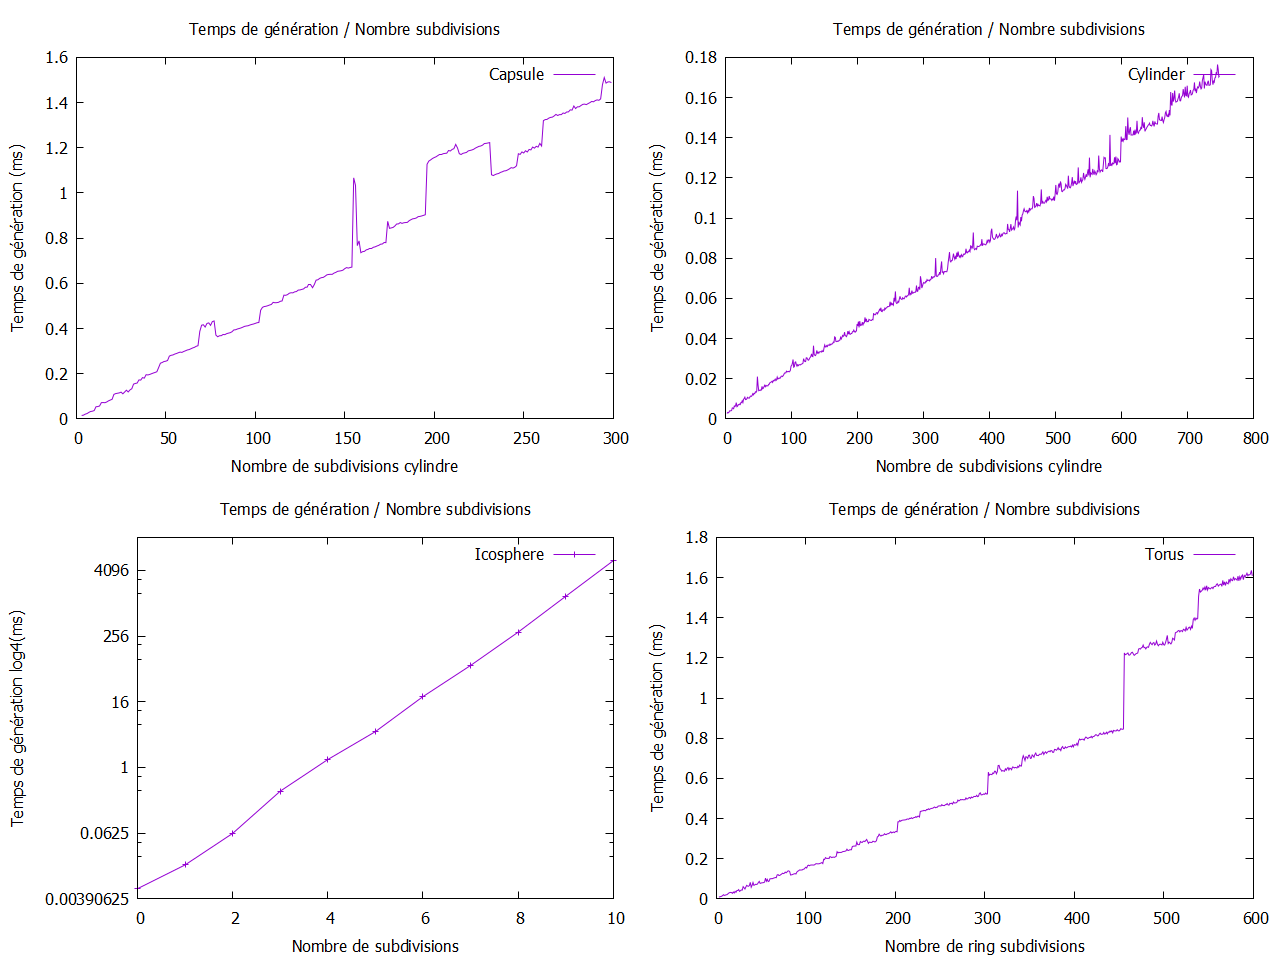
\includegraphics[width=1\textwidth]{Captures/allBenchmarks.png}}

	\caption{Temps de génération pour les maillages simples implémentés en fonction du nombre de subdivisions}
\end{figure}
\FloatBarrier

Toutes les primitives à l'exception de l'icopshère évoluent en temps linéaire quand leur nombre de subdivisions 
augmente et c'est le comportement auquel on pourrait s'attendre. L'icosphère évolue en $4^n$ avec $n$ le nombre 
de subdivisions (le graphique de l'icosphère a son axe des ordonnées en échelle logarithmique base 4). C'est 
également ce à quoi on s'attend puisque la subdivision dyadique multiplie par 4 le nombre de triangles à chaque subdivision.

Les courbes montrent des "accidents", elles ne sont pas totalement "lisses" et cela est dû à différents aspects techniques tels
que la taille des caches du CPU, les réallocations des \textit{std::vector} lors de \textit{push\_back()}, ...


\section {Accessibilité et occlusion ambiante}

\end{document}
